\documentclass[12pt]{article}
\usepackage{tikz}
\usepackage{pgfplots}
\pgfplotsset{compat=1.18}

\begin{document}

\section*{Shading Test 1: Simple axial shade}


\begin{tikzpicture}
  % Simple axial shading: left=red, right=blue
  \shade[left color=red, right color=blue] (0,0) rectangle (5,3);
\end{tikzpicture}

\section*{Shading Test 2: Radial shade}

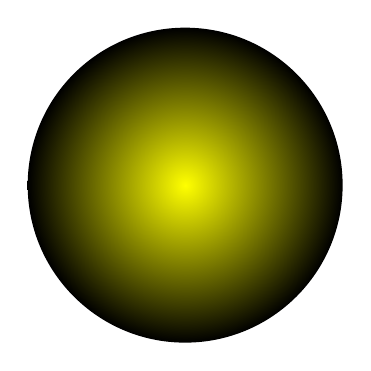
\begin{tikzpicture}
  % Simple radial shading: inner=yellow, outer=black
  \shade[inner color=yellow, outer color=black] (0,0) circle (2);
\end{tikzpicture}

\section*{Shading Test 3: Ball shade}

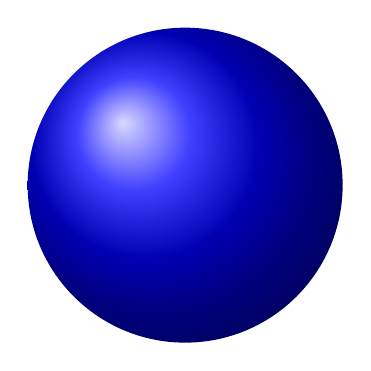
\begin{tikzpicture}
  % Ball shading
  \shade[ball color=blue] (0,0) circle (2);
\end{tikzpicture}

\section*{Shading Test 4: Axis shading (pgfplots)}

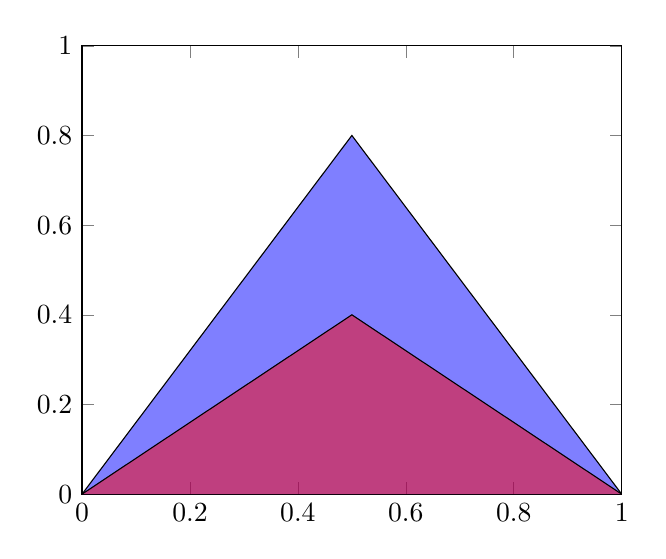
\begin{tikzpicture}
  \begin{axis}[xmin=0, xmax=1, ymin=0, ymax=1]
    \addplot[fill=blue, fill opacity=0.5] coordinates {(0,0) (0.5,0.8) (1,0)};
    \addplot[fill=red, fill opacity=0.5] coordinates {(0,0) (0.5,0.4) (1,0)};
  \end{axis}
\end{tikzpicture}

\section*{Shading Test 5: Multiple color stops}

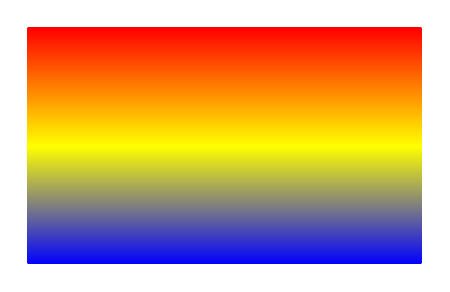
\begin{tikzpicture}
  % Multi-color shading
  \shade[top color=red, bottom color=blue, middle color=yellow]
    (0,0) rectangle (5,3);
\end{tikzpicture}

\end{document}
